\section{Techniques}

This section gives an overview of different techniques used in our crawler. We first show how we integrated a headless web browser into the harvesting process to support blogs that use JavaScript to display page content. The overall software architecture will then be discussed, introducing the Scrapy framework and the enrichments we implemented for our specific use case. Finally we will talk about deployment to scalable, fault resilient distributed architecture.


%%%%%%%%%%%%%%%%%%%%%%%%%%%%%%%%%
\subsection{JavaScript rendering}
% Introduction
JavaScript is a widely used language for client-side web scripting. While some applications simply use it for aesthetics (menus, animations...), an increasing number of websites use JavaScript to download and display content. In such cases, traditional HTML based crawled do not see web pages as they are presented to a human visitor and might therefore be obsolete for data extraction.

% Motivation
In our experiments crawling the blog sphere, we encountered several blogs where data was missed because of the lack of JavaScript interpretation. The most frequent cases where blogs using the Disqus \cite{disqus2013} and LiveFyre \cite{livefyre2013} comment hosting services. These tools are very handy to setup for web-masters because the entire comments infrastructure is externalized and the setup essential comes down to including a JavaScript snippet in each target page. Both of these services heavily rely on JavaScript to download and display the comments, even providing functionalities such as real-time updates for edits and newly written comments. Less commonly, some blogs are fully rendered using JavaScript. When loading such website, the web browser will not receive the page content as an HTML file, but will instead have to execute JavaScript code to download and display the page content. The Blogger platforms provides as a default templates the \emph{Dynamic Views}, which use this mechanism \cite{antinharasymiv2011}.

% The solution
To support blogs with JavaScript generated content, we embed a full web browser into the crawler. After considering multiple option, we opted for PhantomJS \cite{phantomjs2013}, a headless web browser with great performances and scripting capabilities. The JavaScript rendering is done as the very first step of web page processing. Extracting blog post articles, comments or medias therefore works equally well on blogs with JavaScript generated content and traditional HTML-only blogs.

% Click click scripting
When the number of comments on a page exceeds a certain threshold, both Disqus and LiveFyre will only load the most recent ones and the stream of comments will end with a \emph{Show More Comments} buttons. As part of the page loading process, we instruct PhantomJS to repeatedly click on these buttons until all comments are loaded. Paths to Disqus and LiveFyre \emph{show more} buttons were manually obtained and are the only non-generic element of our extraction stack which will require human intervention to maintain and extend to other commenting platforms.


%%%%%%%%%%%%%%%%%%%%%%%%%
\subsection{Architecture}

\begin{figure}
  \capstart
  \centering
  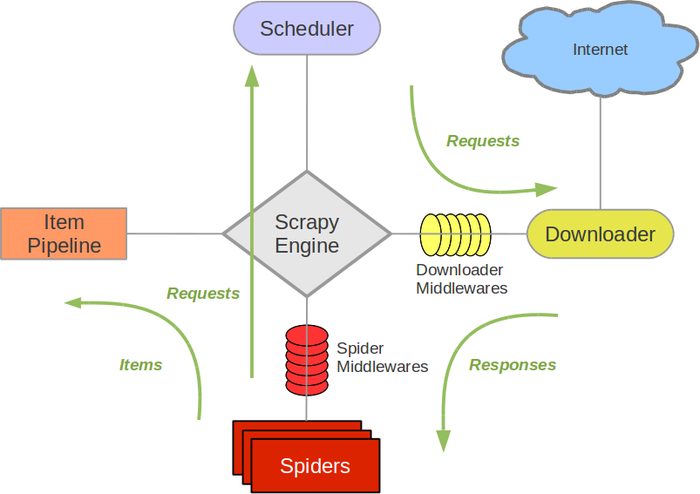
\includegraphics[width=0.47\textwidth]{img/scrapy_architecture.png}
  \caption{Overview of the crawler architecture.\\(Credit: Pablo Hoffman, Daniel Graña, \cite{scrapy2013})}
  \label{architecture}
\end{figure}

Our crawler is built on top of Scrapy \cite{scrapy2013}, an open source Python framework for web crawling. Scrapy provide an elegant and modular architecture illustrated in Figure~\ref{architecture}. Several components can be plugged in Scrapy core infrastructure: \emph{Spiders}, \emph{Item Pipelines}, \emph{Downloader Middlewares} and \emph{Spider Middlewares}; each allowing to implement a different type of functionalities.

Our use case has two types of spiders: \emph{NewCrawl} and \emph{UpdateCrawl}, which respectively implement the logic to crawl a new blog and to get updates from a previously crawled blog. After beeing downloaded and identified as blog posts (details in \ref{enrichingscrapy}), pages are packed into \emph{Items} and sent through the following pipeline of operation:
\begin{enumerate}[noitemsep]
  \item Render JavaScript
  \item Extract content
  \item Extract comments
  \item Download medias
  \item Propagate resulting records to the back end
\end{enumerate}
This pipeline design provides great modularity. Indeed, disabling JavaScript rendering or plugging in an alternative back-end can be done by editing a single line of code.


%%%%%%%%%%%%%%%%%%%%%%%%%%%%%
\subsection{Enriching Scrapy}\label{enrichingscrapy}
% into
In order to identify web pages as blog posts, our implementation enriches Scrapy with two components to narrow the extraction process to the subsets of blog pages holding blog posts: \emph{blog post identification} and \emph{download priority heuristic}.

% blog post identification
Given an entry point to a website, the default Scrapy behavior looks over all pages of the same domain in a \emph{last-in-first-out} manner. The \emph{blog post identification} function is able to identify from an URL whether or not the corresponding page is a blog post. Internally, this function uses a per blog regular expression constructed from web feed entry URLs. This simple approach requires that blogs use the same pattern for all posts (or false negative will occur) which has to be distinct for non-post pages (or false positive will occur). In practice this assumption held for all blog platforms we encountered and seems to be a common practice among web developer.

% download priority heuristic
In order to efficiently deal with blogs with a large number of non-blog-post pages, this \emph{blog post identification} mechanism is not sufficient. Indeed, after all pages identified as blog post are processed, the crawler needs to download non-blog-post pages to search for additional blog posts. To replace the naive random walk, depth first search or breadth first search web site traversals, we use a priority queue where new URL priorities are determined by a simple machine learning algorithm. Given an URL, the machine learning system does an estimation on the number of links to blog post the corresponding page will contain. This estimated number of links are then used as \emph{download priorities} to decide the best URL to visit next. Each time a page is effectively downloaded, the actual number of blog post links it contains is computed and passed to the machine learning system as training data will then be taken into account during future predictions. This mechanism has shown to be indispensable for blogs hosting on the single domain a large number of non-blog web pages, such as a forum or a wiki.

\TODO{Give more details: this function implements a string score predictor using a the Distance-Weighted k-Nearest-Neighbor classifier, as described in \cite{dudani1976} http://ieeexplore.ieee.org/xpls/abs\_all.jsp?arnumber=5408784 This predictor can be used as an active machine learning algorithm by feeding it little by little with new url/score as they are discovered.}

%%%%%%%%%%%%%%%%%%%%%%%%
\subsection{Scalability}
When aiming to work with a large number of inputs, it is crucial to build every layer of the system with scalability in mind \cite{thereactivemanifesto2013}. The BlogForever crawler, and in particular the two core procedures \emph{NewCrawl} and \emph{UpdateCrawl}, are designed to be usable as part of an event-driven, scalable and fault resilient distributed system.

To achieve this property we made the key design choice to have both \emph{NewCrawl} and \emph{UpdateCrawl} as stateless components. From a high level viewpoint, these two components are \emph{purely functional}:
%
\newcommand\URL{\mathbb{U}\text{RL}}
\newcommand\DATE{\mathbb{D}\text{ATE}}
\newcommand\RECORD{\mathbb{R}\text{ECORD}}
\begin{equation*}
  \begin{split}
    NewCrawl:    &~ \URL \rightarrow \mathcal{P}(\RECORD)\\
    UpdateCrawl: &~ \URL \times \DATE \rightarrow \mathcal{P}(\RECORD)
  \end{split}
\end{equation*}
Where $\URL$, $\DATE$ and $\RECORD$ are respectively the set of all URLs, dates and records, and $\mathcal{P}(\cdot)$ designates the powerset. By delegating all shared mutable state to the back end system (Invenio's database), web crawler instances can be added, removed, and used interchangeably.
